\section{Versuchsbeschreibung}
In diesem Versuch wird der Zerfall von Positronium untersucht. Als Quelle für die Positronen dient eine dünne Mylarfolie mit ${}^{22}Na$, welche sich in einer Gaskammer befindet. Der Stickstoff in der Kammer dient einerseits zur Thermalisierung der Positronen, bietet andererseits aber auch Elektronen für die Paarbildung. Im ersten Versuchsteil untersuchen wir den Zwei- und Drei-Photonen-Zerfall, im zweiten Versuchsteil ermitteln wir aus dem Quenching des Triplettzustandes die Aufspaltung durch Zeeman- und Annihilationskraft.

\subsection{Zerfallscharakteristik}

\begin{figure}[H]
 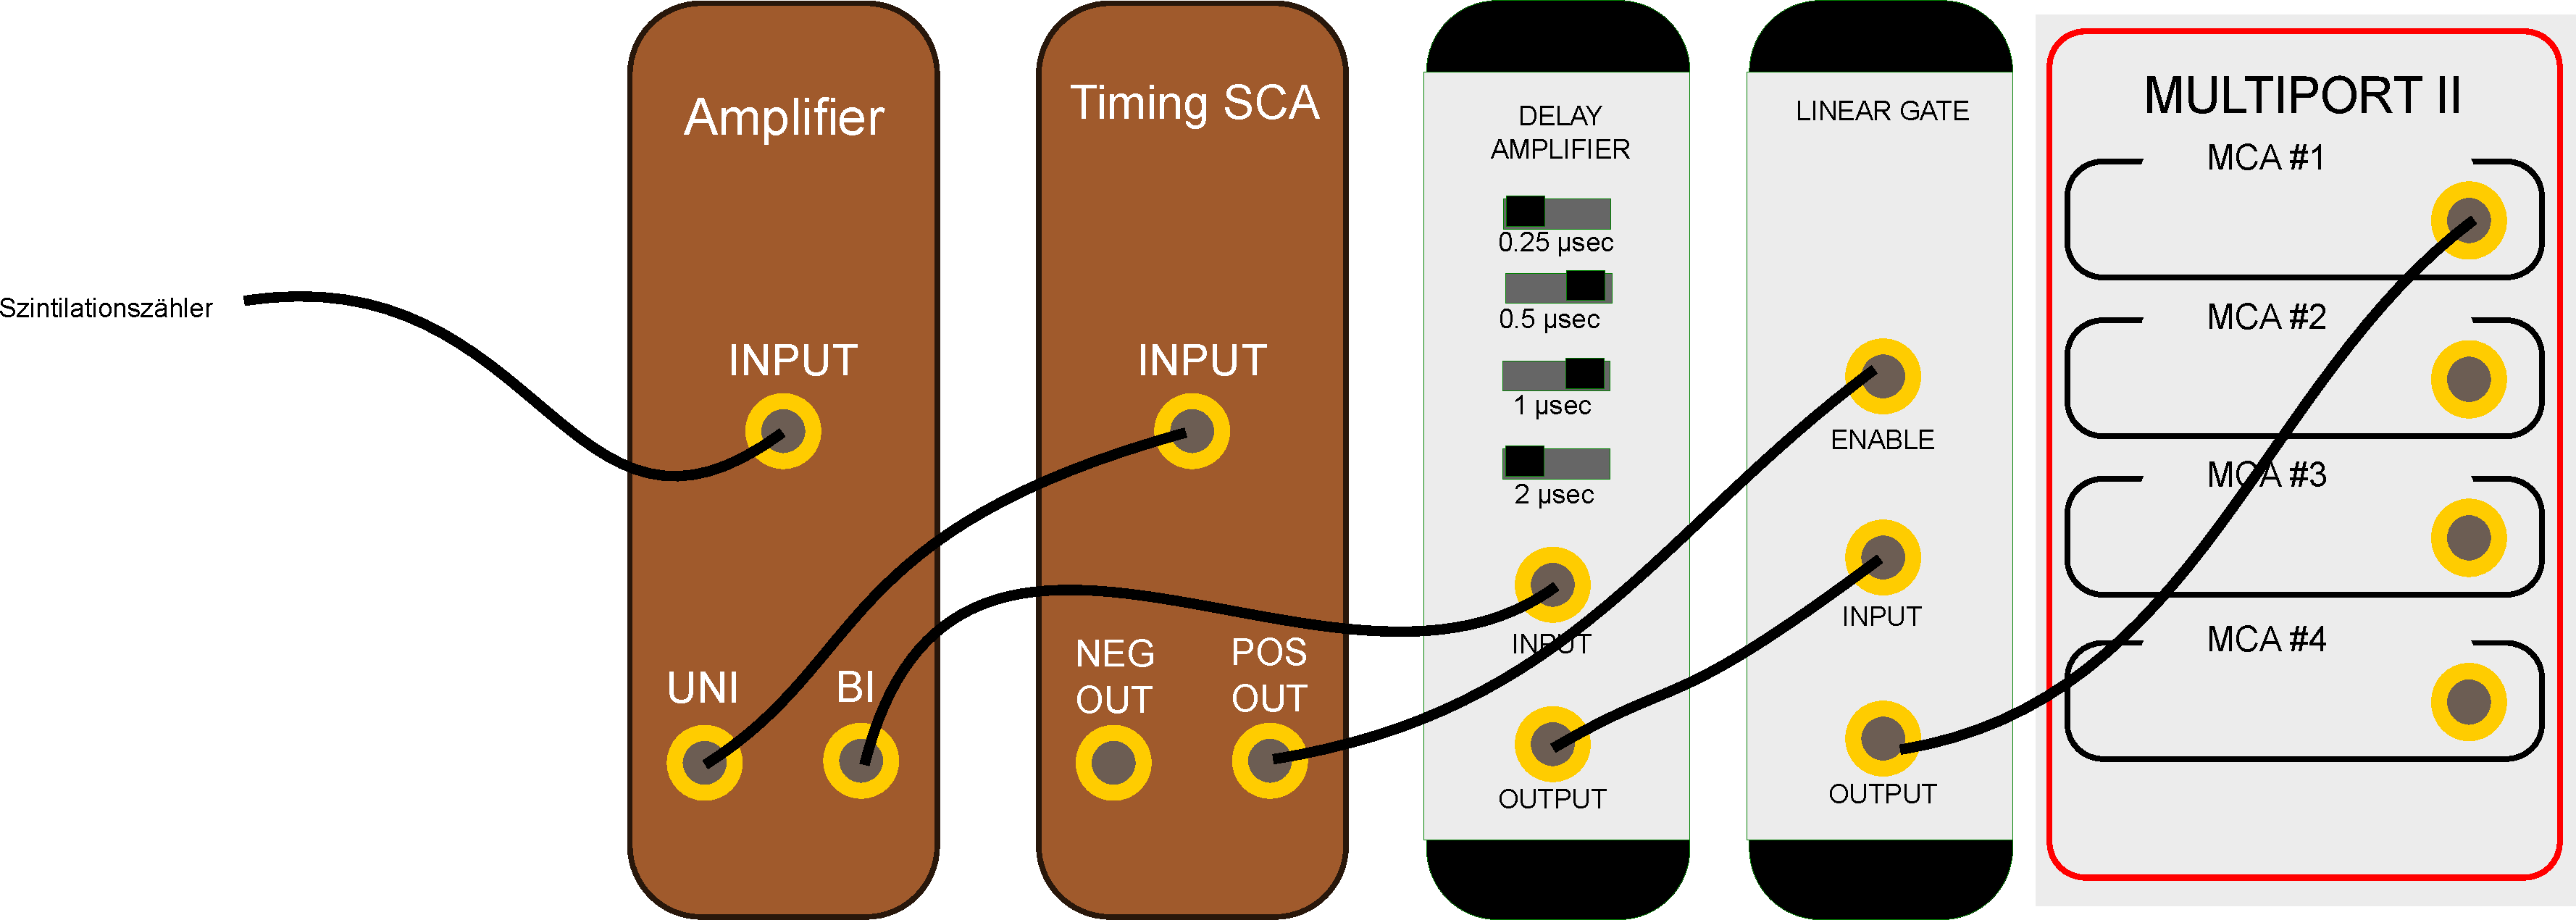
\includegraphics[width=\textwidth]{BilderAufbau/spektrum.pdf}
 \caption{Versuchsaufbau für die Messung des Spektrums und das Einstellen der Fenster}
 \label{schaltplan_sca_lin_mca}
\end{figure}

Das Zerfallsspektrum des Positroniums wird von Szintillatoren gemessen. Zur Energiekalibration wird das komplette Spektrum mit einem Multi Channel Analysator (MCA) aufgenommen. Über den 1270keV Peak des ${}^{22}Na$-Zerfalls und den 511keV Peak des Zwei-Photonen-Zerfalls kann dann eine Energieeichung des MCA ermittelt werden. Da sich die Szintillatoren verschiedene Charakteristiken zeigen, wird diese für alle durchgeführt.

\begin{figure}[H]
 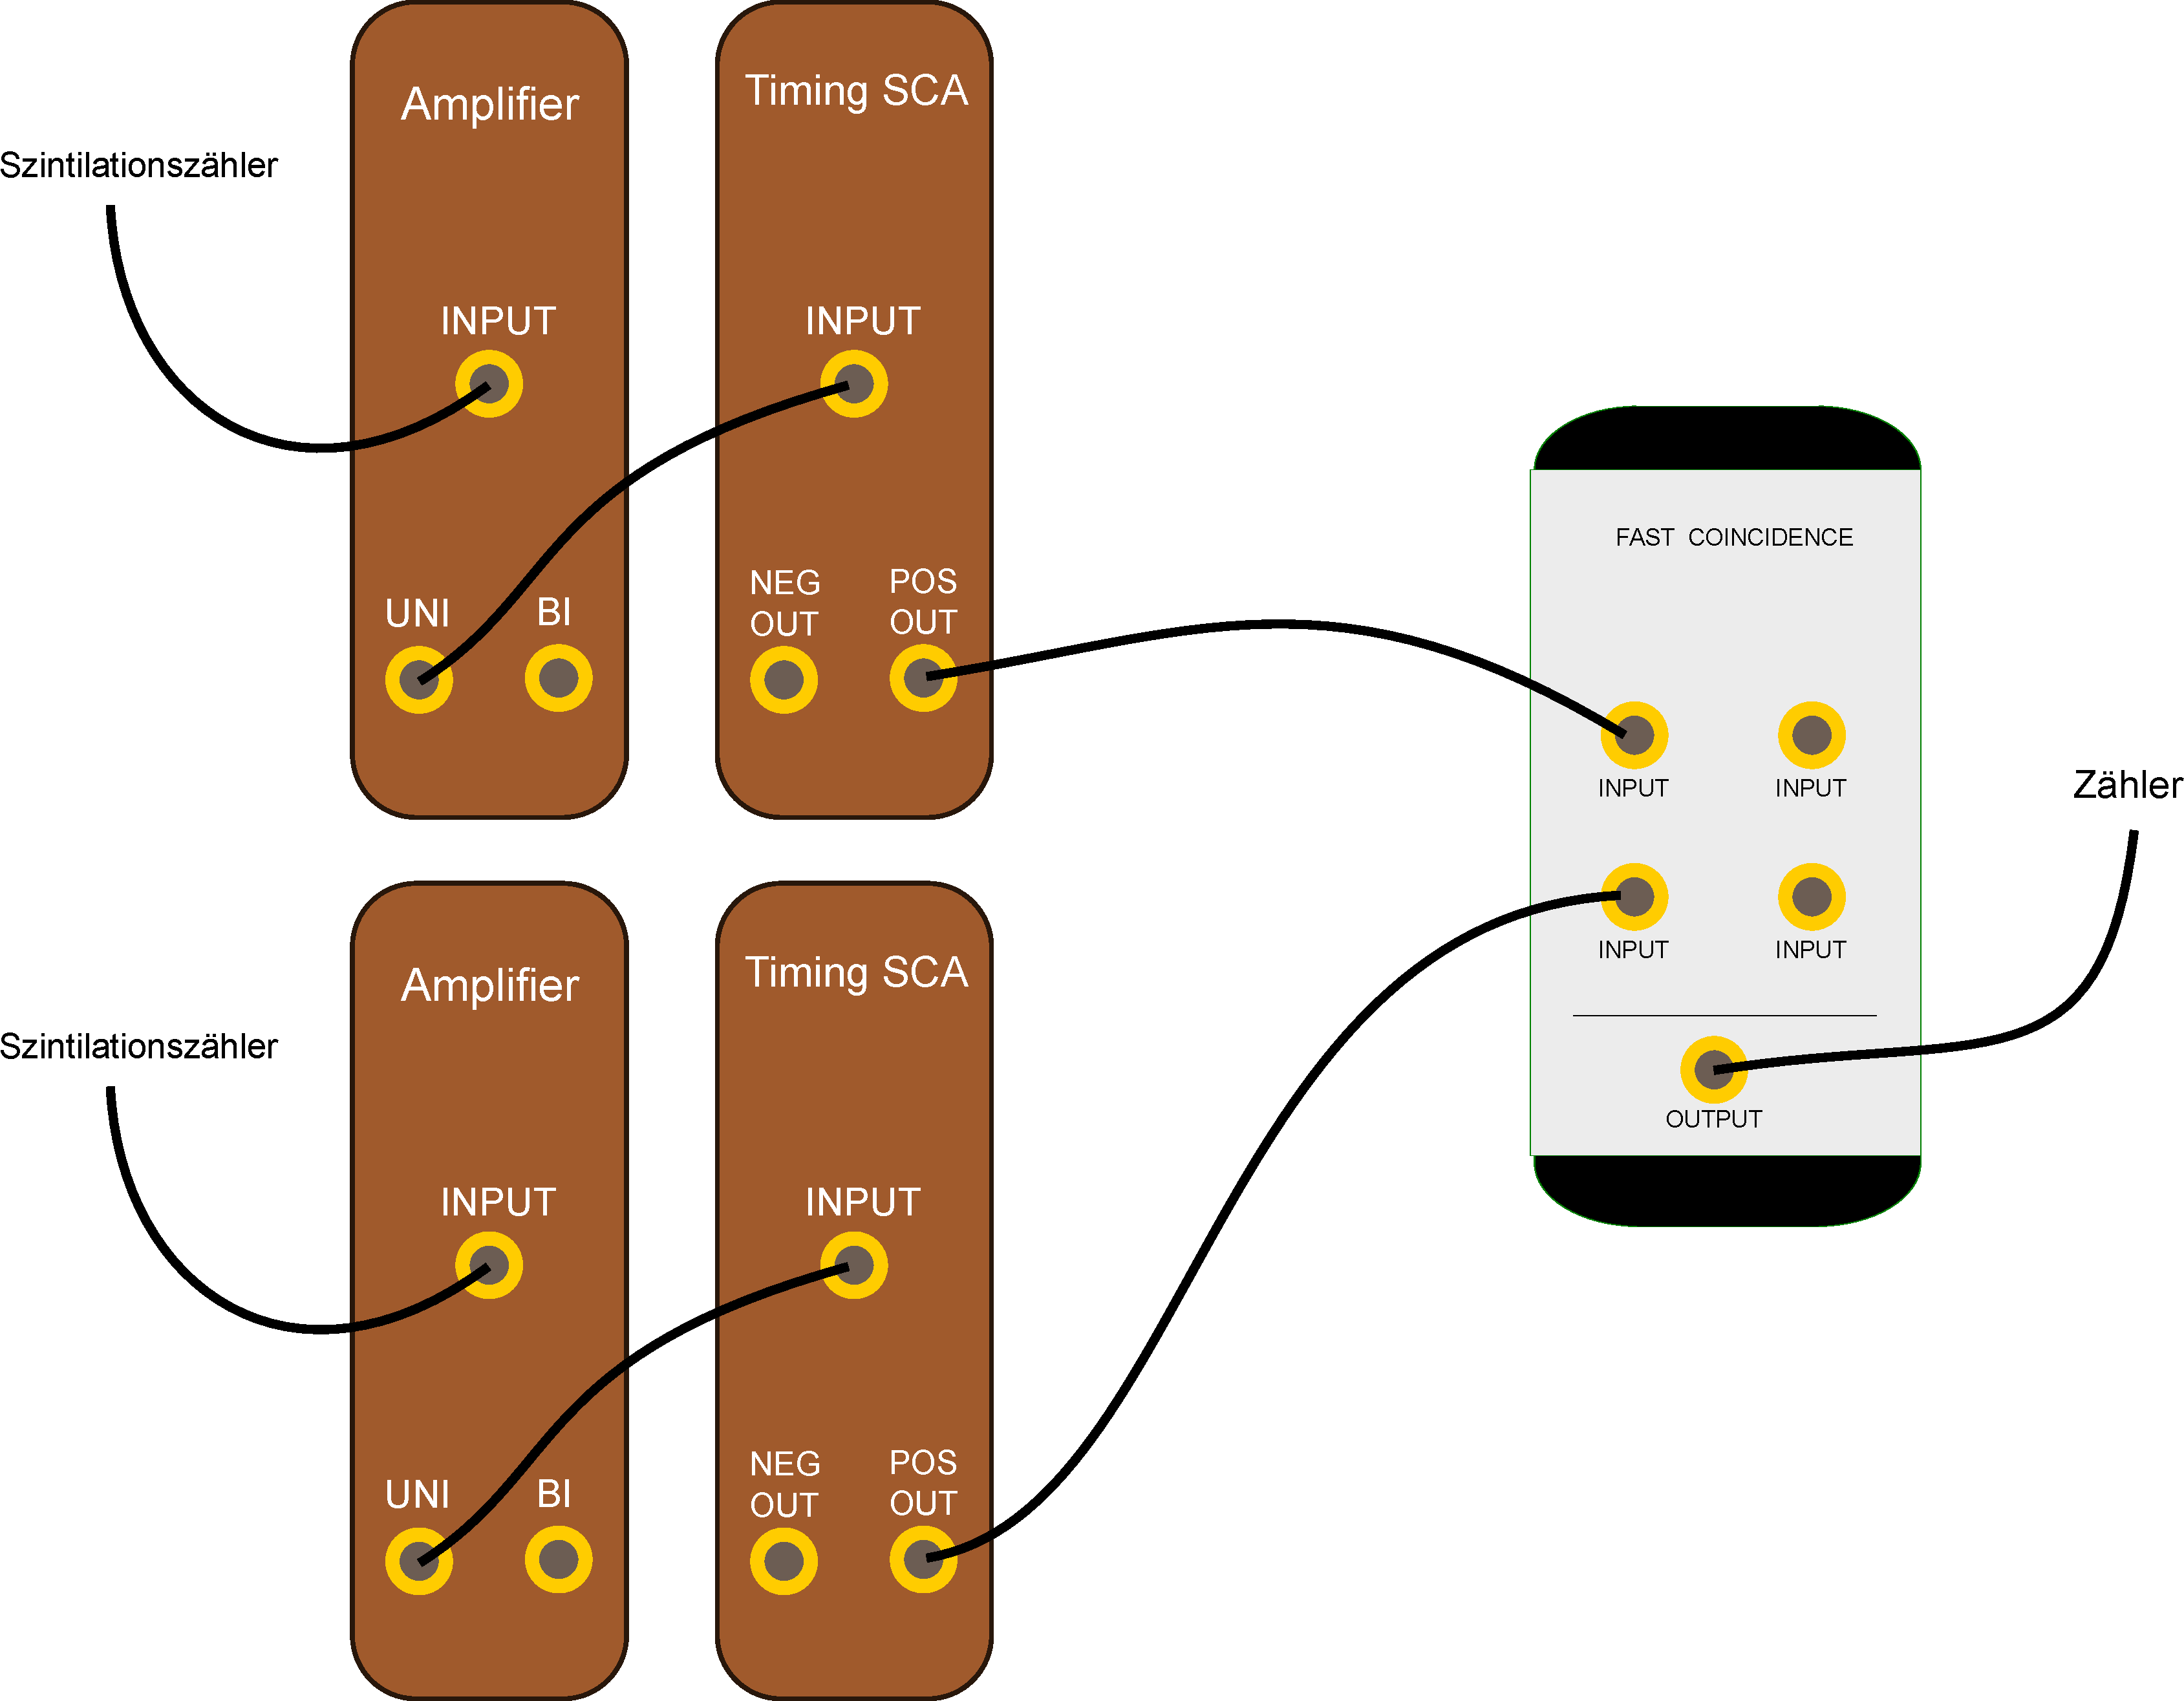
\includegraphics[width=\textwidth]{BilderAufbau/2er-koinzidenz.pdf}
 \caption{Versuchsaufbau für die Koinzidenzmessung des 2-Photonen-Zerfalls}
 \label{schaltplan_2_sca_coin_zaehler}
\end{figure}

Für die Untersuchung des Zerfalls des Singulett-Zustandes wird die Messung auf den 511keV-Peak begrenzt. Zwei der Szintillatoren werden nun in einer Ebene gegeneinader verdreht, um so die Winkelkorrelation zu untersuchen. Dabei werden die Signale zuerst mit Single Channel Analysatoren (SCA) auf den 511keV Bereich begrenzt. Mit einer Fast Coincidenze wird dann überprüft, ob beide Pulse vom selben Zerfall stammen. Die Anzahl solcher Ereignisse innerhalb eines Messintervalls wird gezählt. 


\begin{figure}[H]
 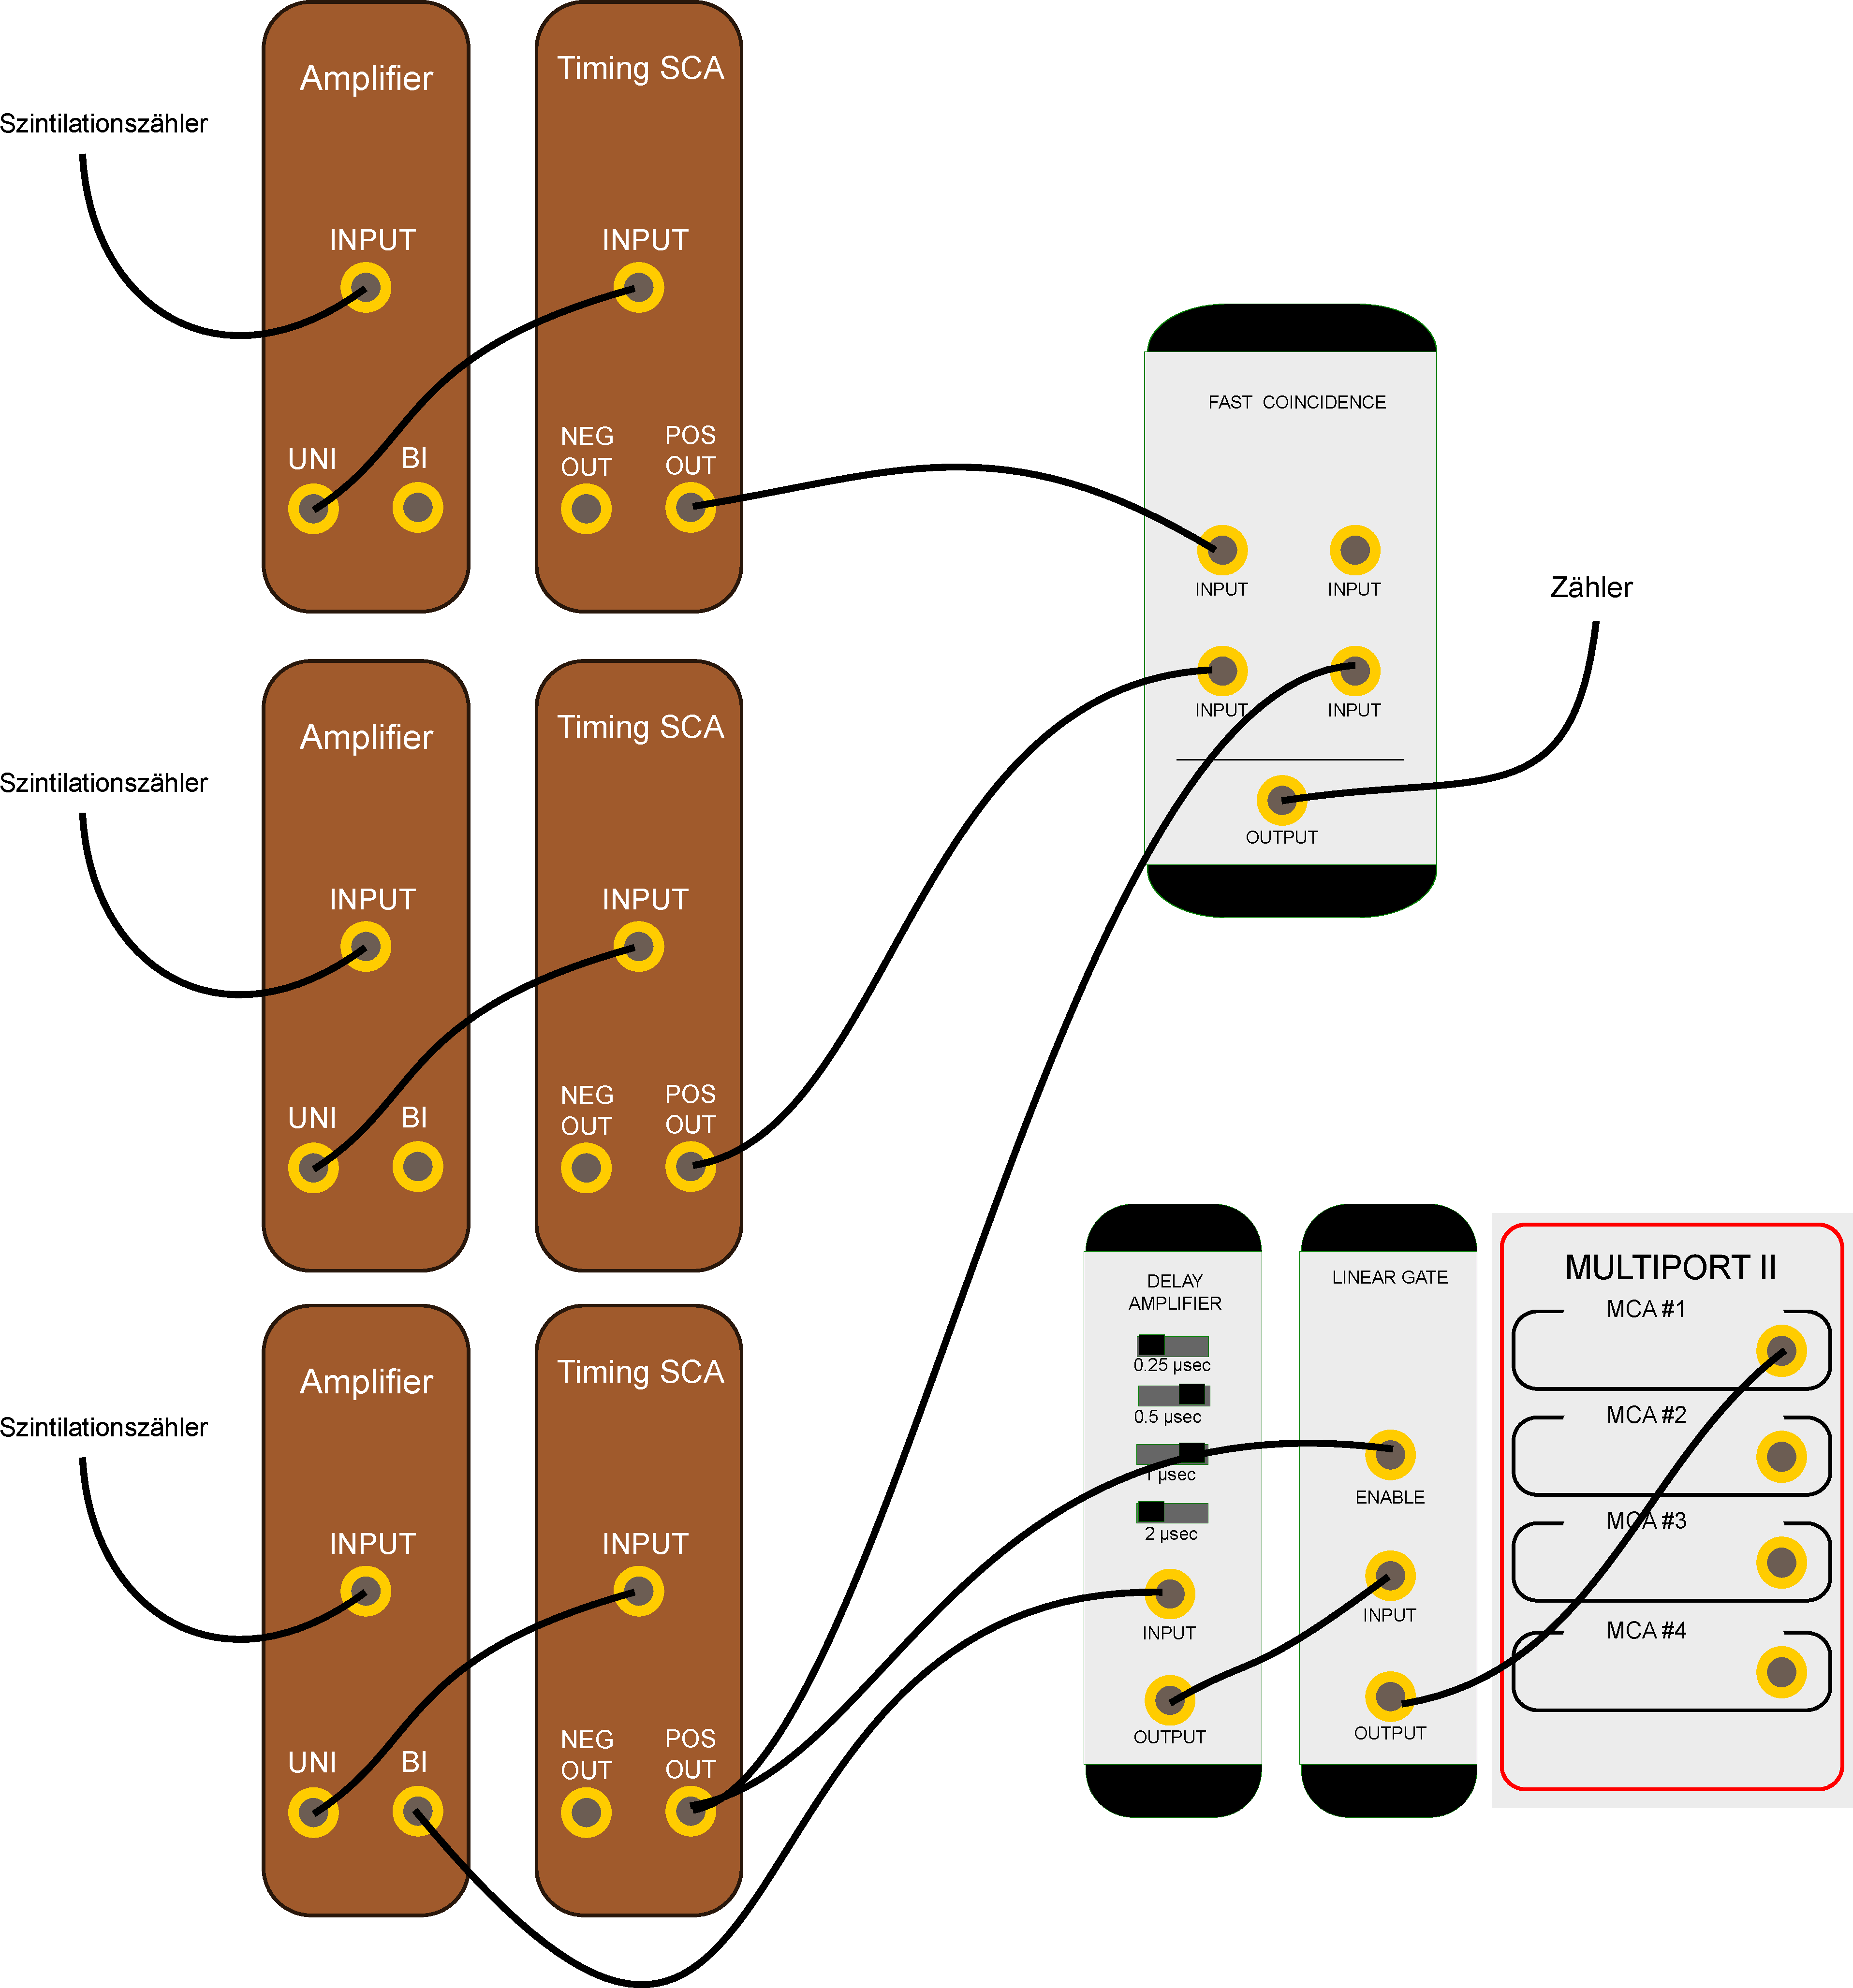
\includegraphics[width=\textwidth]{BilderAufbau/3er-koinzidenz.pdf}
 \caption{Versuchsaufbau für die Koinzidenzmessung des 3-Photonen-Zerfalls}
 \label{schaltplan_3_sca_coin_mca_zaehler}
\end{figure}

Für die Untersuchung des Drei-Photonen-Zerfalls werden drei Szintillatoren in eine $120^\circ$ Konfiguration gebracht. Bei Zweien wird mit SCAs eine Energieobergrenze unterhalb der 511keV des Singulett-Zerfalls gesetzt. Die Energie des dritten Szintillators wird nicht eingeschränkt. Mit der Fast Coinzidence wird überprüft, ob die Photonen vom selben Ereignis stammen. Das Spektrum des dritten SZ wird mit dem MCA aufgenommen. 

\subsection{Quenching}

Im zweiten Versuchsteil geht es darum die Unterdrückung des ${}^3S_0$-Zustandes durch ein Magnetfeld, genannt Quenching, zu untersuchen. Dazu wird jetzt auch beim dritten SCA ein Energiefenster von ca. $\frac{2}{3} m_0$ eingestellt. Mit einem Helmholzspulenpaar wird in der Gaskammer ein konstantes Magnetfeld erzeugt. Dieses wird über die Messreihen variiert und die Abnahme der 3er-Zerfälle registriert.